\documentclass[xcolor=svgnames,dvipsnames,table, hyperref=pdftex, mathserif, presentation]{beamer}
\usepackage{amsmath,amssymb,amsfonts,amsthm}
\usepackage{ctex}
\usepackage{graphics}
\usepackage{graphicx}
\usepackage{xcolor}
\usepackage{wasysym}
\usepackage{bbm}
\usepackage{url}
\usepackage{beamerleanprogress}
\usepackage{tikz-dependency}
\usepackage{tikz-qtree}
\usepackage{multirow}

\newcommand{\tabincell}[2]{\begin{tabular}{@{}#1@{}}#2\end{tabular}}%放在导言区
\usetheme{CambridgeUS}
%\usetheme{Pittsburgh}
\usecolortheme{orchid} % seahorse  orchid rose
\setbeamertemplate{blocks}[rounded][shadow=true]
\AtBeginSection[]{%
  \begin{frame}<beamer>
    \frametitle{Outline}
      \tableofcontents[current] 
    \end{frame}
  \addtocounter{framenumber}{-1}% If you don't want them to affect the slide number
}
\AtBeginSubsection[]
{
  \begin{frame}
  \frametitle{Outline}
    \tableofcontents[currentsection,currentsubsection]
  %\tableofcontents[sectionstyle=show/hide,subsectionstyle=hide/show/hide]
  \end{frame}
  \addtocounter{framenumber}{-1}% If you don't want them to affect the slide number
}
\newcommand{\setof}[1]{\ensuremath{\left \{ #1 \right \}}}
\newcommand{\tuple}[1]{\ensuremath{\left \langle #1 \right \rangle }}
\newcommand{\red}[1]{\textcolor{red}{#1}}
\newcommand{\brown}[1]{\textcolor{brown}{#1}}
\newcommand{\green}[1]{\textcolor{green}{#1}}
\newcommand{\blue}[1]{\textcolor{blue}{#1}}
\newcommand{\cyan}[1]{\textcolor{cyan}{#1}}

%gets rid of navigation symbols
\setbeamertemplate{navigation symbols}{}

\begin{document}

\title[Paraphrase]{Paraphrase Identification}

\institute[icst@pku]{
  
}
\author[Zhe Han]{\\ Zhe Han \\ 1401214342\\ iampkuhz@gmail.com
}

\frame[t,plain]{ \titlepage } % [t,plain]

\frame{
  \frametitle{ Outline  }
  
   \begin{itemize}

  \item 算法流程
    \begin{itemize}
      \item 特征选择
      \item 特征效果
      \item 分类器说明
    \end{itemize}

  \item 分析总结
    \begin{itemize}
    \item 实验效果
    \item 分析
    \end{itemize}
  \end{itemize}

}

\frame{
  \frametitle{Process}
  \begin{itemize}
   \item 流程
      \begin{itemize}
       \item 提取句子lexical, semantic features (precision, recall, normal form/lemma form)
	  \begin{itemize}
	   \item lexical: 相同单词, 相同单词对, 编辑距离, 最大公共子串, 
	   \item semantic: 相似/不同的POS tagger分布, N/V单词相似度, 命名实体相似度分布, dependency relation类型分布, dependency relation pair 相似度
	   \item 所有判断单词是否相似都采用WordNet::Synset.Similarity
	  \end{itemize}
	  
	\item 将特征转换为weka要求的文件格式
	\item 调用weka的系统分类器训练模型
	    \begin{itemize}
	     \item 在开发集(扩展到400维)上测试效果, 选取最好的组合分类器(voting)作为最终的分类器
	    \end{itemize}
	\item 使用选定的组合分类器在扩展的训练集(train + dev)训练模型
	\item 在测试集上跑分类结果
      \end{itemize}

  \end{itemize}

}

\frame{
    \frametitle{feature select}
    \begin{itemize}
     \item 实现了下面三篇文章的大多数特征
     \item 利用第三篇的思想: 多个分类器投票(+0.4\% compared with SVM only)
    \end{itemize}

  \begin{block}{paper}
  \begin{itemize}
   \item \begin{footnotesize}
          (75.6\%)Using dependency-based features to take the "para-farce" out of paraphrase
         \end{footnotesize}

   \item \begin{footnotesize}
          (75.0\%)Using machine translation evaluation techniques to determine sentence-level semantic equivalence
         \end{footnotesize}

   \item \begin{footnotesize}
          (76.6\%)Paraphrase identification on the basis of supervised machine learning techniques
         \end{footnotesize}
 
  \end{itemize}
  \end{block}
}

\frame{
    \frametitle{feature select}
    \begin{itemize}
     \item common words
	\begin{itemize}
	 \item common words precision: 统计第一句话里重复单词的频率
	 \item common words recall: 统计第二句话里重复单词的频率
	\end{itemize}
     \item Position-independent word error rate(precision, recall)
	\begin{itemize}
	 \item 和 common words 正好相反,统计每句话里不同单词的概率
	\end{itemize}
    \item proper name(4 dimension, precision, recall)
	\begin{itemize}
	 \item 对句子做命名实体识别(stanford ner),对于 4 类,分别求每句话中每一类的单词的重复出现的概率
	\end{itemize}

    \end{itemize}

}


\frame{
    \frametitle{feature select}
    \begin{itemize}
     \item POS distribute vector
     \begin{figure}[h]
  \centering
  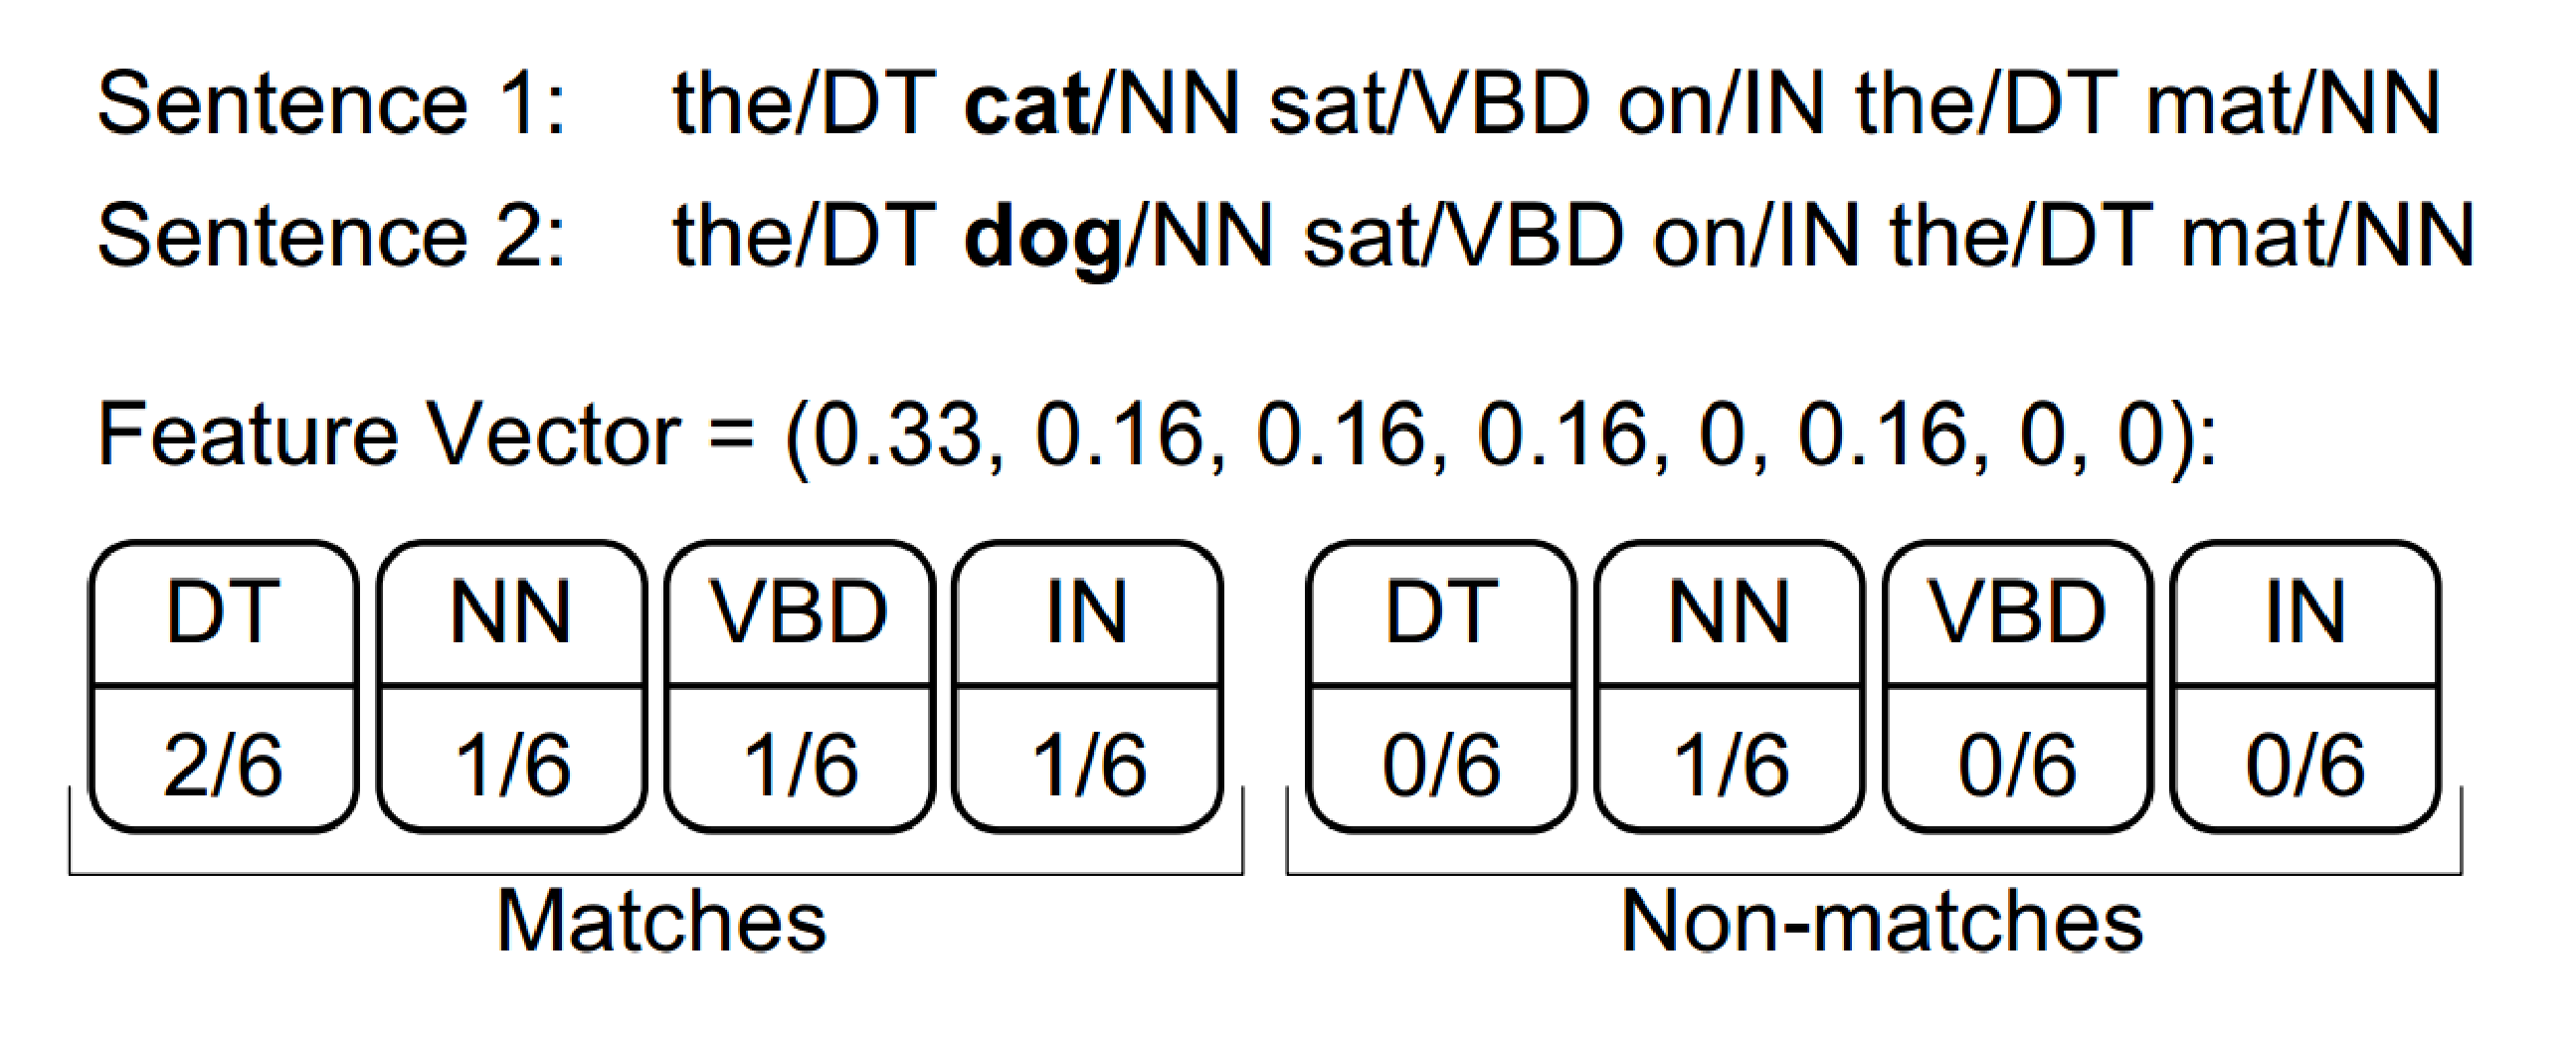
\includegraphics[width=0.6\textwidth]{POSvector}
  \end{figure}
  
    \item skip-gram common words
	\begin{itemize}
	 \item 句子的任意两个单词组成的单词对(距离小于等于 4), 考虑另一句话中是否有相同配对(距离小于等于 4), 计算重复单词对数
	\end{itemize}
     
     \item noun/verb similarity
	\begin{itemize}
	 \item 对句子先做词性标注,然后统计其中名词和动词的重复率
	\end{itemize}

    \end{itemize}
    
}

\frame{
    \frametitle{feature select}
    \begin{itemize}
     \item dependency relation distribution ( 88 dimension)
	\begin{itemize}
	 \item 类似于 POS distribute vector。Stanford parser 一共有 44 种关系,前 44 维表示相同关系的分布频率,后 44 维表示不同关系的分布频率。
	\end{itemize}
    \item dependency relation lemma word
	\begin{itemize}
	 \item 使用 lemmatization 之后的句子, 分析relation pair的相似概率
	\end{itemize}

    \end{itemize}

}

\frame{
    \frametitle{feature list}
    
    
    \begin{tiny}
    \rowcolors{2}{red!5}{red!20}
    %\begin{table*}[htb]\footnotesize
     \begin{tabular}{|c|c|c|c|}
    \hline
     \textbf{feature} & accuracy & \textbf{feature} & accuracy \\ \hline
     common words & 69.9\% & common lemma words &  72.6\% \\ \hline
     edit distance & 69.8\% & lemma sentence edit distance & 70.4\% \\ \hline
     skip-gram common words &70.3\% &  skip-gram common lemma words &70.9\% \\ \hline
     longest common subsequence& 70.2\% & longest common lemma subsequence & 72.3\% \\ \hline
     noun/verb similarity &69.7\% &  noun/verb lemma similarity & 69.7\% \\ \hline
     proper name(4 dimension)&73.9\% &  proper lemma name(4 dimension) &73.5\% \\ \hline
     dependency relation pair& 69.1\% &  dependency relation lemma pair &68.6\% \\ \hline
     \tabincell{c}{dependency relation distribution \\ (88 dimension) } & 70.7\%&  \multicolumn{2}{c| }{ }\\ \hline
     \tabincell{c}{dependency relation lemma distribution \\ (88 dimension) } & 69.8\%&  \multicolumn{2}{c| }{ }\\ \hline
     dependency relation distribution)& 70.7\% &  \multicolumn{2}{c| }{ }\\ \hline
     dependency relation lemma word& 70.0\% &  \multicolumn{2}{c| }{ }\\ \hline
     POS distribute vector(72 dimension) & 73.2\% &  \multicolumn{2}{c| }{ }\\ \hline
     POS distribute lemma vector(72 dimension) & 72.05\% &  \multicolumn{2}{c| }{ }\\ \hline
     Position-independent word error rate(PER) &70.7\% &  \multicolumn{2}{c| }{ }\\ \hline
     Position-independent lemma word error rate(PER) & 73.4\% &  \multicolumn{2}{c| }{ }\\ \hline
    \end{tabular}
    %\end{table*}
  \end{tiny}
    

}

\frame{
    \frametitle{Classifier}
    \begin{itemize}
     \item accuracy on single classifier
    \end{itemize}

     \rowcolors{2}{red!5}{red!20}
     \begin{tabular}{|c|c|}
      \hline
     \textbf{classifier} & accuracy \\ \hline
     SVM & 76.8\% \\ \hline
     LibLINEAR & 76.6\% \\ \hline
     SPegasos & 76\% \\ \hline
     SimpleLogistic & 75.6\% \\ \hline
     VotedPerceptron & 74.7\% \\ \hline
     J48 & 68.4\% \\ \hline
     KNN & 67.9\% \\ \hline
     NaiveBayes & 67.4\% \\ \hline
     RBFNetwork & 66.9\% \\ \hline
     
     \end{tabular}


}
\frame{
    \frametitle{Summary}
    \begin{itemize}
     \item 优点
	\begin{itemize}
	 \item Accuracy 高
	    \begin{itemize}
	     \item 高于三篇参考文章, 只略低于statte-of-art(77.4\%)
	    \end{itemize}
	 \item trick很少, 不需要交叉验证找参数
	    \begin{itemize}
	     \item 只采用weka的默认分类函数, 没有训练特别参数
	    \end{itemize}
	\item 特征覆盖面广
	    \begin{itemize}
	     \item lexical, POS tag, NER, dependency, word semantic(WordNet), .. 
	    \end{itemize}

	\item 提升了求解速度
	    \begin{itemize}
	     \item HashMap存储POStagged sentence, lemmatized sentence, POStagged lemmatized sentence. 一次计算, 之后直接调用
	     \item 不加dependency feature, 程序在十几秒内得到结果; 加入dependency feature, 在8分钟左右
	    \end{itemize}

	\end{itemize}

    \end{itemize}

}

\frame{
    \frametitle{Summary}
    \begin{itemize}
     \item 缺点
	\begin{itemize}
	 \item 特征可能冗余(不漂亮)
	    \begin{itemize}
	     \item 特征太多. 将所有正确的特征加入, 没有实验是否冗余
	     \item 写了一个算法, 对所有多维的特征, 遍历(取/不取), 时间有限没有跑
	    \end{itemize}
	\item 句子级别的语义信息抽取很不好
	    \begin{itemize}
	     \item 没有真正的提取到句子的信息..
		 \item \red{Socher(2011NIPS) :  Dynamic pooling and unfolding recursive autoencoders for paraphrase detection}
		 \item wordvec + R(ecusive)NN + dynamic polling: 4类特征, 76.8\%

	     
	    \end{itemize}

	\end{itemize}

    \end{itemize}

}
\frame{
  \frametitle{方法概述}
  
  \subtitle{paper}{
  \begin{center}\Large paper\\ \end{center}
  \begin{block}{paper}
  \begin{itemize}
   \item \begin{footnotesize}
          Using dependency-based features to take the "para-farce" out of paraphrase
         \end{footnotesize}

   \item \begin{footnotesize}
          Using machine translation evaluation techniques to determine sentence-level semantic equivalence
         \end{footnotesize}

   \item \begin{footnotesize}
          Paraphrase identification on the basis of supervised machine learning techniques
         \end{footnotesize}

   \item \begin{footnotesize}
          vector machines for paraphrase identification and corpus construction
         \end{footnotesize}
 
  \end{itemize}
  \end{block}

  }                                                 
}

\end{document}
